%%%%%%%%%%%%%%%%%%%%%%%%%%%%%%%%%%%%%%%%%%%%%%%%%%%%%%%%%%%%%%%%%%%%%%%%%%
%																		%
%	Plantilla Latex para presentación del proyecto de curso				%
%	Programación de Aplicaciones para Internet y la Nube					%
%																		%
%	Creada por: Duván Pardo, Wilson López								%
%																		%
%	Versión: 0.1															%
%	Dapardoc@gmail.com ; Wilrilo@gmail.com								%
%																		% 
%	Se requieren los archivos plantilla.bbl y							% 
%	El directorio Imagenes que contiene: CECAD,DC, Elementos y RITA		%  
%																		%
%%%%%%%%%%%%%%%%%%%%%%%%%%%%%%%%%%%%%%%%%%%%%%%%%%%%%%%%%%%%%%%%%%%%%%%%%%

\documentclass[10pt]{article}\usepackage[]{graphicx}\usepackage[]{color}
%% maxwidth is the original width if it is less than linewidth
%% otherwise use linewidth (to make sure the graphics do not exceed the margin)
\makeatletter
\def\maxwidth{ %
  \ifdim\Gin@nat@width>\linewidth
    \linewidth
  \else
    \Gin@nat@width
  \fi
}
\makeatother

\definecolor{fgcolor}{rgb}{0.345, 0.345, 0.345}
\newcommand{\hlnum}[1]{\textcolor[rgb]{0.686,0.059,0.569}{#1}}%
\newcommand{\hlstr}[1]{\textcolor[rgb]{0.192,0.494,0.8}{#1}}%
\newcommand{\hlcom}[1]{\textcolor[rgb]{0.678,0.584,0.686}{\textit{#1}}}%
\newcommand{\hlopt}[1]{\textcolor[rgb]{0,0,0}{#1}}%
\newcommand{\hlstd}[1]{\textcolor[rgb]{0.345,0.345,0.345}{#1}}%
\newcommand{\hlkwa}[1]{\textcolor[rgb]{0.161,0.373,0.58}{\textbf{#1}}}%
\newcommand{\hlkwb}[1]{\textcolor[rgb]{0.69,0.353,0.396}{#1}}%
\newcommand{\hlkwc}[1]{\textcolor[rgb]{0.333,0.667,0.333}{#1}}%
\newcommand{\hlkwd}[1]{\textcolor[rgb]{0.737,0.353,0.396}{\textbf{#1}}}%

\usepackage{framed}
\makeatletter
\newenvironment{kframe}{%
 \def\at@end@of@kframe{}%
 \ifinner\ifhmode%
  \def\at@end@of@kframe{\end{minipage}}%
  \begin{minipage}{\columnwidth}%
 \fi\fi%
 \def\FrameCommand##1{\hskip\@totalleftmargin \hskip-\fboxsep
 \colorbox{shadecolor}{##1}\hskip-\fboxsep
     % There is no \\@totalrightmargin, so:
     \hskip-\linewidth \hskip-\@totalleftmargin \hskip\columnwidth}%
 \MakeFramed {\advance\hsize-\width
   \@totalleftmargin\z@ \linewidth\hsize
   \@setminipage}}%
 {\par\unskip\endMakeFramed%
 \at@end@of@kframe}
\makeatother

\definecolor{shadecolor}{rgb}{.97, .97, .97}
\definecolor{messagecolor}{rgb}{0, 0, 0}
\definecolor{warningcolor}{rgb}{1, 0, 1}
\definecolor{errorcolor}{rgb}{1, 0, 0}
\newenvironment{knitrout}{}{} % an empty environment to be redefined in TeX

\usepackage{alltt}   			% Describe el tipo de documento, y el tamaño de la letra del texto

\usepackage[utf8]{inputenc}				% Define codificación para que permita caracteres latinos (acentos)
\usepackage[spanish,activeacute]{babel} 	% Paquete para poder escribir con tildes y otros caracteres especiales

\usepackage{vmargin}						% Código para margenes y formato de página
\setpapersize{A4}
\setmargins	{2.2cm}     					% margen izquierdo
{1 cm}                 		% margen superior
{16.5cm}               		% anchura del texto
{23.42cm}             		% altura del texto
{20pt}                		% altura de los encabezados
{1.2cm}               		% espacio entre el texto y los encabezados
{0pt}                		% altura del pie de página
{2cm}                 		% espacio entre el texto y el pie de página

\usepackage{amsmath}						% paquete para expresiones matemáticas
\usepackage{amsfonts}					% paquete para escritura de ecuaciones 
\usepackage{amssymb}						% paquete para caracteres especiales para ecuaciones 

\usepackage{fancyhdr}					% Temas para encabezado y pie de pagina
\usepackage{fancyvrb}
\pagestyle{fancy} 

\pagenumbering{arabic} 					% Numeración de paginas {arabic roman}
\usepackage{hyperref}					% Para hipervinculos
\usepackage{graphicx}					% Para incluir imágenes
\usepackage{ float}
\usepackage{caption}						% Descripciones de las figuras
\usepackage{subcaption}					% Descripción varias imagenes en usa sola figura
\graphicspath{ {Imagenes/} }				% Directorio de imágenes esta capeta va donde esta el archivo tex


\usepackage{color, colortbl}				% Colores para tablas
\usepackage{listings}					% Para el código Fuente
\usepackage{xcolor}						% para color en codigos o listrings
\definecolor{limegreen}{RGB}{50,100,50}	% Definición de colores ejemplo verde en RGB
\definecolor{Red}{RGB}{220,120,120}		% se definen colores para la tabla en el cronograma 
\definecolor{LightCyan}{rgb}{0.88,1,1}
\definecolor{azul}{RGB}{120,120,210}

%para pytohn
\DeclareFixedFont{\ttb}{T1}{txtt}{bx}{n}{9} % for bold
\DeclareFixedFont{\ttm}{T1}{txtt}{m}{n}{9}  % for normal
\definecolor{deepblue}{rgb}{0,0,0.5}
\definecolor{deepred}{rgb}{0.6,0,0}
\definecolor{deepgreen}{rgb}{0,0.5,0}

\newcommand\pythonstyle{\lstset{
		language=Python,
		basicstyle=\ttm,
		otherkeywords={self},             % Add keywords here
		keywordstyle=\ttb\color{deepblue},
		emph={MyClass,__init__},          % Custom highlighting
		emphstyle=\ttb\color{deepred},    % Custom highlighting style
		stringstyle=\color{deepgreen},
		frame=tb,                         % Any extra options here
		showstringspaces=false            % 
	}}
	
	
	% Python environment
	\lstnewenvironment{python}[1][]
	{
		\pythonstyle
		\lstset{#1}
	}
	{}
	
	% Python for external files
	\newcommand\pythonexternal[2][]{{
			\pythonstyle
			\lstinputlisting[#1]{#2}}}
	
	% Python for inline
	\newcommand\pythoninline[1]{{\pythonstyle\lstinline!#1!}}


%%%%
\lstdefinestyle{base}{
	language=C,
	emptylines=1,
	breaklines=true,
	showspaces=fasle,
	showstringspaces=false,
	extendedchars=true,
	basicstyle=\ttfamily\color{black},
	moredelim=**[is][\color{limegreen}]{'}{'}, 	% Para este caso especial el caracter ' y & encierran
	moredelim=**[is][\color{blue}]{&}{&},		% un fragmento de código que quiere ser coloreado
}

\lstset{numbers=left, numberstyle=\tiny, stepnumber=2, numbersep=5pt}

	\definecolor{dkgreen}{rgb}{0,0.6,0}
	\definecolor{gray}{rgb}{0.5,0.5,0.5}
	\definecolor{mauve}{rgb}{0.58,0,0.82}
	
	\lstset{frame=tb,
		language=R,
		aboveskip=3mm,
		belowskip=3mm,
		showstringspaces=false,
		columns=flexible,
		numbers=none,
		keywordstyle=\color{blue},
		numberstyle=\tiny\color{gray},
		commentstyle=\color{dkgreen},
		stringstyle=\color{mauve},
		breaklines=true,
		breakatwhitespace=true,
		tabsize=3
	}


%Aquí inicia el documento.
\IfFileExists{upquote.sty}{\usepackage{upquote}}{}
\begin{document}
	% Se define el Encabezado
	%clhead[]{Proyecto}
	\lhead[]{Programación de Aplicaciones para Internet y la Nube}
	\rhead[]{\textbf{2016-I}}
	\renewcommand{\headrulewidth}{0.5pt}
	
	\thispagestyle{empty}						% La primera página no lleva estilo (sin encabezado)
	\begin{center}
		\large {Programación de Aplicaciones para Internet y la Nube
			\hspace{5 cm}\textbf{2016-I}}
		\bigskip  
		\textbf{
			\LARGE{\\Sistema para adquisición de datos para el control y supervisión de cultivos domésticos por protocolo IPV6}}\\								% Nombre del proyecto
	\end{center}	
	\begin{flushright}	
		\bigskip	
		Nombre del Estudiante: \textbf{Wilson López}			% Nombre del estudiante
	\end{flushright} 
	
	\section{Introducción}
	
	La problemática ambiental que enfrenta el mundo, debido al crecimiento exponencial de las ciudades, donde el área forestal ha sido reducida casi por completo varios países del mundo han creado políticas locales y nacionales con el fin de concientizar a la sociedad acerca de la importancia del agro y la forestación, para enfrentar los efectos del cambio climático. En el caso particular de Colombia el ministerio de agricultura tiene  leyes para el desarrollo científico e investigativo en el campo de la agricultura  y desarrollo rural \cite{ministerioagricultura} ,Se puede presentar como caso particular el desarrollo de techos verdes en el acuerdo 418 de 2009, la Secretaría de Ambiente ha desarrollado la campaña “Una piel natural para Bogotá” esta dicta capacitaciones y asesorías de forma gratuita para quienes deseen implementar estas tecnologías en el distrito. \cite{ley}.
	\\
	
	Un techo verde es un sistema constructivo que permite mantener de manera sostenible un paisaje vegetal sobre la cubierta de un inmueble mediante la adecuada integración entre el inmueble intervenido, la vegetación escogida, el medio de crecimiento diseñado y los factores climáticos y ambientales. \cite{techoverde}
	
	\begin{figure}[ht] % Es preferible verificar la documentación para que la imagen quede correctamente segun el parámetro entre []
		\centering
		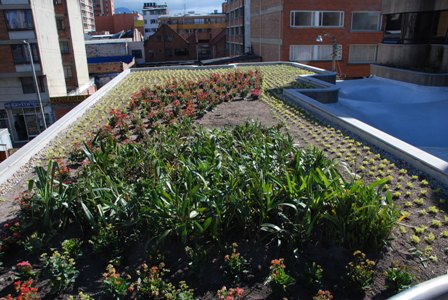
\includegraphics[scale=2.5]{techoverde}   % Scale se utiliza para cambiar el tamaño de la imagen
		\caption{Terraza piso 3 Secretaria Distrital de Ambiente}
		
	\end{figure}
	
	La importancia que tiene hoy en día tomar conciencia sobre los techos verdes y los cultivos domésticos y conectividad a Internet que tiene la mayoría de los dispositivos que nos rodean debido a la conciencia que se esta generando hoy en día de techos verdes y cultivos domestico y la introducción  de Internet de las cosas (IoT) en este campo(\cite{cultivo}). el proyecto de curso busca tener control sobre estos cultivos por medio de un sistemas de adquisición de datos que tenga conectividad Ipv4 y IPv6 (\cite{ipv6}) que se pueda conectar a un  servidor web donde se puedan visualizar las variables de los sensores
	
	
	
	
	\section{Descripción del proyecto}
	
	El proyecto está enmarcado en la temática de Internet de las Cosas (IoT) y  Wireless Sensor Networks (WSNs), para el control y supervisión  de los cultivos domésticos. El objetivo principal del proyecto es adquirir datos de diferentes sensores( humedad y temperatura) para controlar las variables medidas. Permitiendo la supervisión de las condiciones de los cultivos propios y de los demás usuarios del sistema, de tal forma que se puedan hacer comparaciones, de esta forma poder hacer comparaciones de diferentes cultivos y posteriormente poder realizar un intercambio de experiencias y  cultivos. \\
	
	
	El proyecto se divide en los siguientes componentes:
	
	\begin{itemize}
		\item \textbf{adquisición de datos:} los datos se simularan por medio de un números aleatorios dentro de la Raspberry
		\item \textbf{actuadores:} por medio de una raspberry pi se controlaran un actuador desde la raspberry y desde la pagina que conecta a la raspberry.
		
		\item \textbf{comunicación IPv6:} En el caso de la comunicación IPv6 se trabajara en la red interna de la universidad dado que IPv6 no esta soportado por nubes privadas como es el caso de amazon. La  raspberry pi soportan IPv6, se plantea apuntar a la direccional IPv6 de alguno de los dispositivos para  adquirir datos  por medio de una pagina   HTML donde se ven los valores de los sensores y se pueda controlar el actuador 
		\item\textbf{ visualización de los datos en la nube:} se plantea subir los datos a el servidor de Ubidots para que los usuarios puedan ver los datos desde lugares externos a la Universidad.
		\item seguridad: Como se trata de un ejercicio educativo y que la aplicación no se centra en la seguridad de los datos  el sistema contara con una seguridad de los datos baja. 	
	\end{itemize}
	
	
	
	
	
	\begin{figure}[h] % Es preferible verificar la documentación para que la imagen quede correctamente segun el parámetro entre []
		\centering
		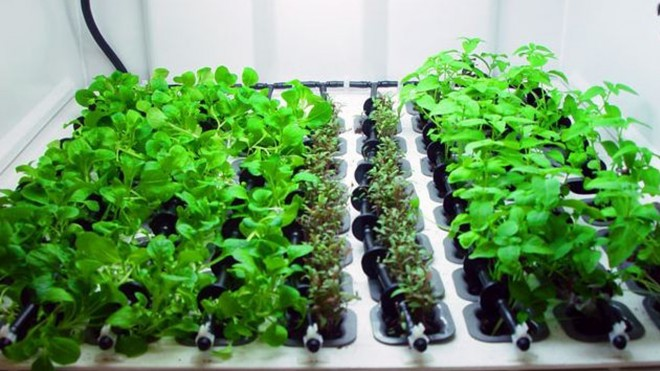
\includegraphics[scale=0.5]{Elementos}   % Scale se utiliza para cambiar el tamaño de la imagen
		\caption{cultivo domestico \textbf{} }
	\end{figure}
	
	
	
	\section{Objetivos}
	
	\subsection{General}
	
	\begin{itemize}
		\item Diseñar y realizar un prototipo de un sistema para adquisición de datos para el control y supervisión de cultivos domésticos por protocolo IPV6
	\end{itemize}
	
	\subsection{Especificos}
	
	\begin{itemize}
		\item diseñar un dispositivo para la adquisición y control de variables (temperatura y humedad)
		\item diseñar he implementar comunicación por IPv6 entre los dispositivos.
		\item Implementar sistema para visualizar los datos adquiridos en la nube 
	\end{itemize}
	
	
	
	\section{Desarrollo del proyecto}	
	
	\subsection{Preparación de la Raspberry}
	
	El primer paso es instalar el sistema operativo NOOBS en la Raspberry. Para la instalación se utiliza una microSD de 8Gb mínimo se descarga la imagen de la pagina de raspberrypi, a través de Internet y se instala dicha imagen en la microSD. (\href{https://www.raspberrypi.org/downloads/noobs/}{https://www.raspberrypi.org/downloads/noobs/}). al finalizar la instalación arranca el SO de raspberrypi  
	
	
	\begin{figure}[ht] % Es preferible verificar la documentación para que la imagen quede correctamente segun el parámetro entre []
		\centering
		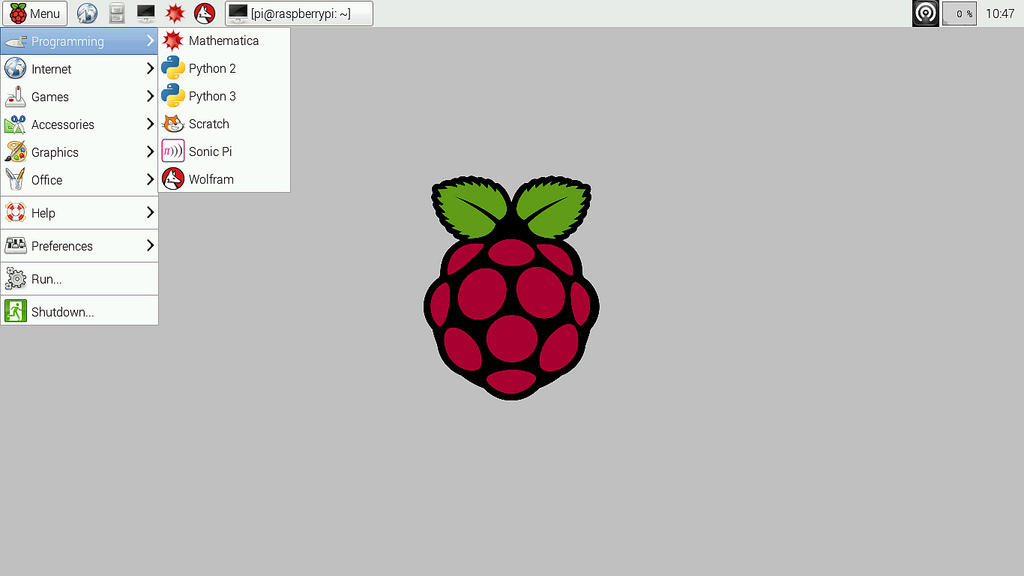
\includegraphics[scale=0.5]{raspbian}   % Scale se utiliza para cambiar el tamaño de la imagen
		\caption{Sistema Operativo de raspberry raspbian}
		
	\end{figure}
	
	Procedemos a instalar los paquetes y programas necesarios para adquirir los datos y mostrarlos por medio de una interfaz HTML por medio de python, para esto abrimos una consola en las raspberry y ejecutamos los siguientes comandos: 
	
			
\begin{small}
			\begin{lstlisting}[frame=single]
		sudo apt-get update
		sudo apt-get upgrade
		sudo apt-get install python
		sudo apt-get install python-dev
		sudo apt-get install libjpeg-dev
		sudo apt-get install libfreetype6-dev
		sudo apt-get install python-setuptools
		sudo apt-get install python-rpi.gpio
		sudo easy_install pip
		sudo pip install ubidots
		
			
			\end{lstlisting}
\end{small}	

Ahora procedemos a descargar e instalar el gestor de paquetes de Python PIP:

\begin{small}
	\begin{lstlisting}[frame=single]
	
sudo apt-get install python-pip
pip install tornado
pip install --upgrade pip
	
	\end{lstlisting}
\end{small}	
	
Con los paquetes instalados podemos iniciar el trabajo, sin embargo se recomienda instalar el paquete $xrdp$  con el comando \texttt{sudo apt-get install xrdp} este controlar la raspberry por medio de un escritorio remoto:	

	\begin{figure}[H] % Es preferible verificar la documentación para que la imagen quede correctamente segun el parámetro entre []
		\centering
		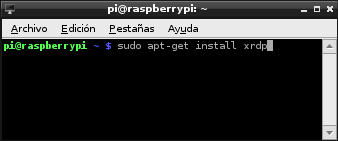
\includegraphics[scale=0.8]{xrdp}   % Scale se utiliza para cambiar el tamaño de la imagen
		\caption{Instalación paquete $xrdp$ (tomado de \href{http://rc-code.blogspot.com.co/2014/02/raspberry-pi-y-windows-conexion-por.html}{http://rc-code.blogspot.com.co/2014/02/raspberry-pi-y-windows-conexion-por.html} )}
		
	\end{figure}
	
Ahora podemos entrar desde otro equipo que se encuentre en la red a ver y controlar el monitor de la raspberry para acceder por defecto, el usuario es pi y la contraseña es raspberry:	



	\begin{figure}[ht] % Es preferible verificar la documentación para que la imagen quede correctamente segun el parámetro entre []
		\centering
		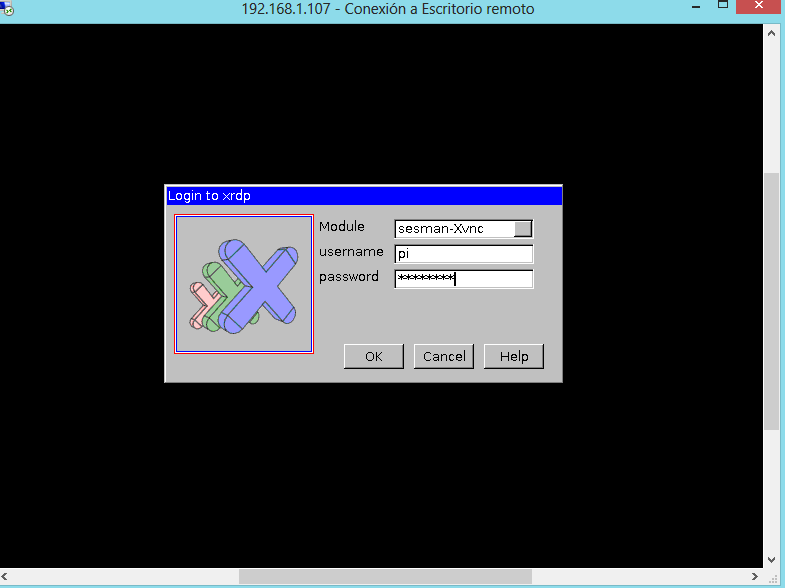
\includegraphics[scale=0.5]{remoto}   % Scale se utiliza para cambiar el tamaño de la imagen
		\caption{Escritorio Remoto $xrdp$ (tomado de \href{http://4.bp.blogspot.com/-tkTJcqk92no/UwZlYu6IEYI/AAAAAAAAAUU/qtcO16PWVCc/s1600/1.png}{http://4.bp.blogspot.com/-tkTJcqk92no/UwZlYu6IEYI/AAAAAAAAAUU/qtcO16PWVCc/s1600/1.png} )}	
	\end{figure}
	
	
\subsection{Ubidots}

Ubidots es un servicio en la nube que permite almacenar y analizar información de sensores en tiempo real. La creación de cuenta es gratuita y permite manejar diferentes variables al mismo tiempo. Comenzamos creando una cuenta en \href{http://ubidots.com/}{ubidots}, cuando este creada entramos a My Profile:

	\begin{figure}[ht] % Es preferible verificar la documentación para que la imagen quede correctamente segun el parámetro entre []
		\centering
		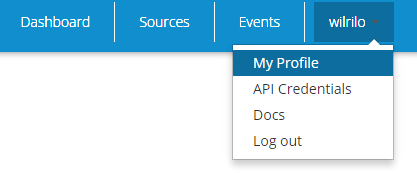
\includegraphics[scale=0.5]{ubi1}   % Scale se utiliza para cambiar el tamaño de la imagen
		\caption{Estructura Ubidots}
		
	\end{figure}

En la Parte Derecha se encuentra un menu llamado "API Keys" dando clic en este menú, tenemos el API Key y Tokens para autentificar nuestra cuenta en la raspberry proceso que se explicara mas adelante   
  
 	\begin{figure}[ht]
 		\centering
 		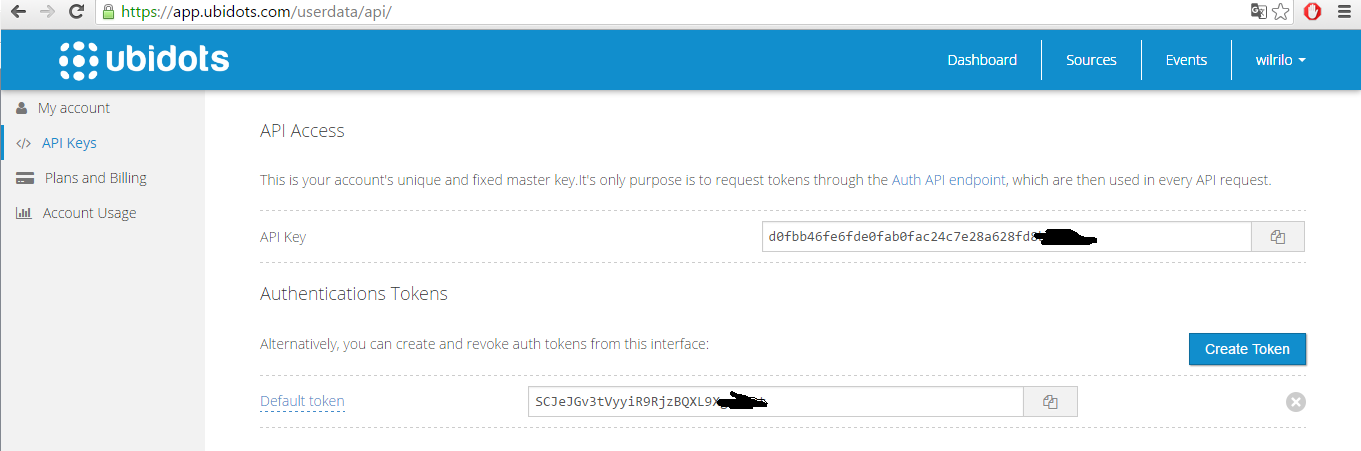
\includegraphics[scale=0.3]{ubi2}   % Scale se utiliza para cambiar el tamaño de la imagen
 		\caption{adquirir API y Token de Ubidots} 		
 	\end{figure}

Ahora procedemos a crear las variables y tomar las ID's de las variables necesarias para subir los datos a la nube. en la parte derecha superior vamos al menú \textit{Sources}, donde agregaremos los diferentes tipos de variables en \textbf{Add Data Soures}, le damos en el signo mas y le damos un nombre a la fuente que acabamos de crear.
  
 	\begin{figure}[ht]
 		\centering
 		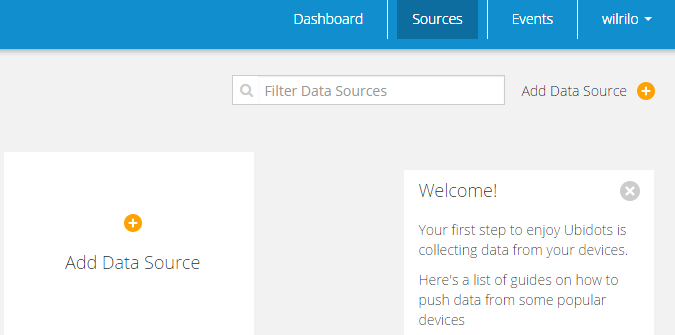
\includegraphics[scale=0.3]{ubi3}   % Scale se utiliza para cambiar el tamaño de la imagen
 		\caption{Agregar Variables en Ubidots} 		
 	\end{figure}  

Al dar clic en la fuente que acabamos de crear encontramos un menú que nos permite crear variables en \textit{Add Variable}, para este caso particular creamos una variable por defecto.

 	\begin{figure}[ht]
 		\centering
 		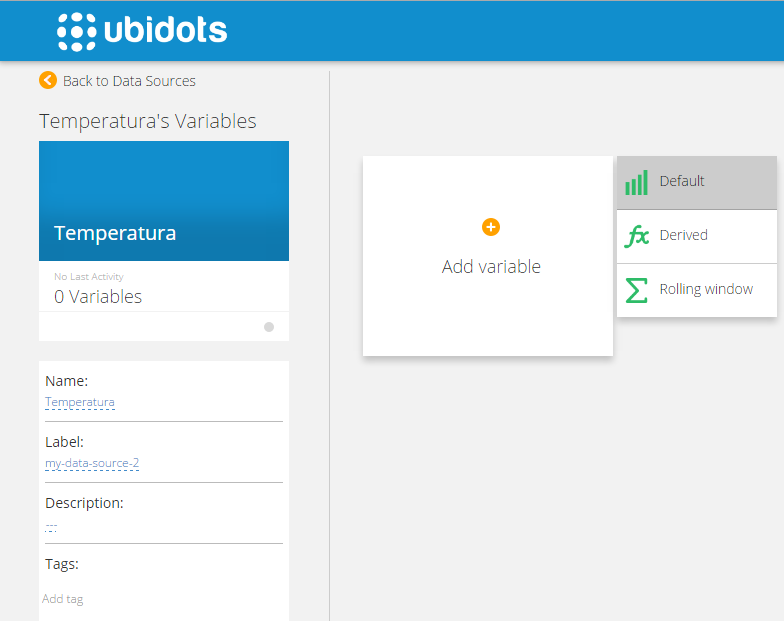
\includegraphics[scale=0.3]{ubi4}   % Scale se utiliza para cambiar el tamaño de la imagen
 		\caption{Creación de variables Ubidots} 		
 	\end{figure}  
	
Al crear variables en la parte superior derecha de cada variable se encuentra un signo de \textit{i} latina damos clic sobre este símbolo nos mostrara el ID de dicha variable la cual sera utilizada en el programa de la raspberry para subir los datos a la nube:

 	\begin{figure}[H]
 		\centering
 		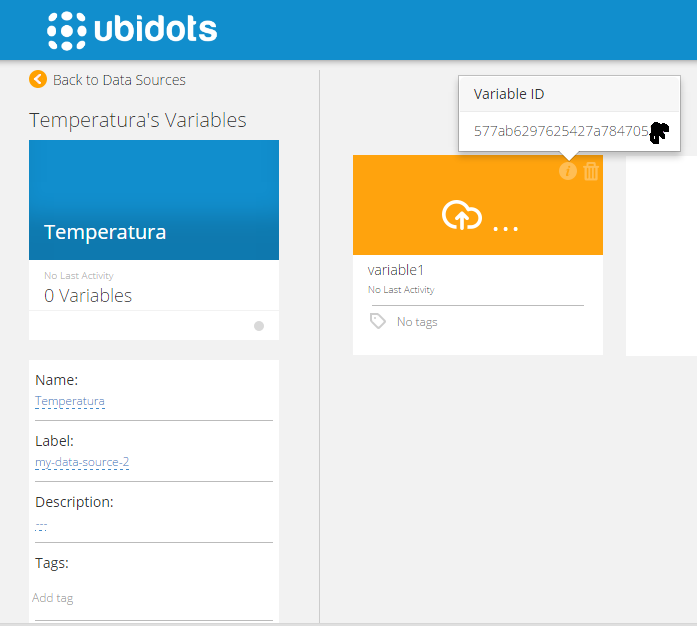
\includegraphics[scale=0.3]{ubi5}   % Scale se utiliza para cambiar el tamaño de la imagen
 		\caption{ID de las variables en Ubidots} 		
 	\end{figure}
 	
Finalmente para el proyecto que se pretende desarrollar creamos dos fuentes de datos Humedad y temperatura cada uno con las variables
 	\begin{figure}[ht]
 		\centering
 		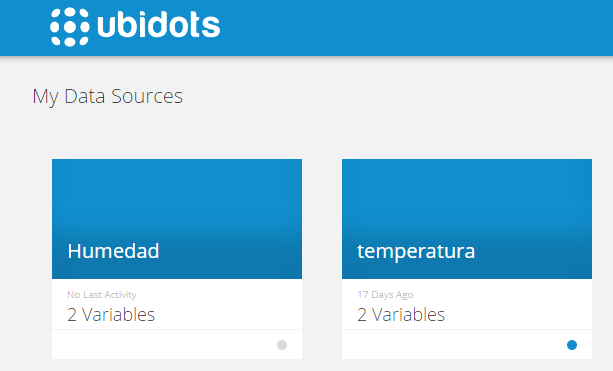
\includegraphics[scale=0.3]{ubi6}   % Scale se utiliza para cambiar el tamaño de la imagen
 		\caption{Variables creadas para el proyecto en Ubidots} 		
 	\end{figure}

  \subsection{Programa en python }
   
   
Para comenzar a trabajar en python es necesario crear la siguiente \href{https://github.com/wilrilo/repo_final_nube/tree/master/repo_final_nube/ProyectoF_Pi}{estructura de archivos}.

	
		\begin{figure}[ht] 
			\centering
			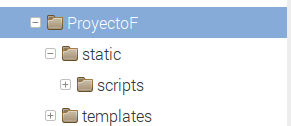
\includegraphics[scale=1]{estructura}   % Scale se utiliza para cambiar el tamaño de la imagen
			\caption{Estructura de archivos para trabajar en python}	
		\end{figure}


		
 En la carpeta \href{https://github.com/wilrilo/repo_final_nube/tree/master/repo_final_nube/ProyectoF_Pi}{proyectoF\_Pi} vamos a crear un archivo llamado  en el estará todo el programa de python, en la carpeta \href{https://github.com/wilrilo/repo_final_nube/tree/master/repo_final_nube/ProyectoF_Pi/templates}{\texttt{templates}} se almacena un archivo llamado \href{https://github.com/wilrilo/repo_final_nube/blob/master/repo_final_nube/ProyectoF_Pi/templates/index.html}{\texttt{index.html}} donde esta el código de la pagina HTML que nos muestra a cualquier usuario que se encuentre en la red los datos de que están adquiriendo y finalmente en la carpeta \href{https://github.com/wilrilo/repo_final_nube/tree/master/repo_final_nube/ProyectoF_Pi/static/scripts}{scripts} que esta dentro de la carpeta static se encuentra el archivo \href{https://github.com/wilrilo/repo_final_nube/blob/master/repo_final_nube/ProyectoF_Pi/static/scripts/raspberry.js}{\texttt{raspberry.js}} el cual configura la pagina HTML la dirección IP y puerto donde se va visualizar:
 \\

 \subsubsection{\textbf{Codigo archivo \href{https://github.com/wilrilo/repo_final_nube/blob/master/repo_final_nube/ProyectoF_Pi/programa.py}{\texttt{programa.py}}:}}

En el archivo se importan las librerías de tornado con el que se crea el servidor HTML, librerías para tener timer en la aplicación. para generar números aleatorios, usar el GPIO de la raspberry y para subir las variables a Ubidots 

\begin{python}
import tornado.web
import tornado.websocket
import tornado.httpserver
import tornado.ioloop
import tornado.options
import json
import time
import threading
import random
from uuid import uuid4
from ubidots import ApiClient	
#libreria para usar el puerto GPIO
import RPi.GPIO as GPIO
\end{python}

Se crean la API y los ID's de Ubidots para poder subir y visualizar las variables en la nube, los  codigos correspondiente al API y los ID's se generan en la pagina de Ubidots proceso que se explica mas adelante. 
 
\begin{python}
# crear api 
api = ApiClient(token= 'SCJeJGv3tVyyiR9RjzBQXL9XgzCCxt')
#creamos las api y los id
humedad = api.get_variable("5763b2ab7625421ca1a7d82a")
temperatura = api.get_variable("5763ac2376254249a1fa9eba")
\end{python}

ahora configuramos los pines para entrada y salida del control de la válvula:
\begin{python}
#pines por el numero canal de las etiquetas.
GPIO.setmode(GPIO.BCM)

#Configurando el pin de salida
GPIO.setup(11, GPIO.OUT)
GPIO.output(11, False)

#Configurando el pin de entrada
swichtPin = 10

GPIO.setup(swichtPin, GPIO.IN, pull_up_down=GPIO.PUD_UP)
\end{python}

Creamos la interrupción por hardware de la valvula:


\begin{python}
def pinkCall(channel):
pulsador = Raspberry()
inputValue = GPIO.input(11)

if(inputValue == True):
GPIO.output(11, False)

pulsador.notifyCallbacks(0, 'La valvula fue apagado por Hardware')

if(inputValue == False):
GPIO.output(11, True)

pulsador.notifyCallbacks(1, 'La valvula fue encendido por Hardware')

print('Interrupcion por hardware')


GPIO.add_event_detect(swichtPin, GPIO.RISING, callback=pinkCall, bouncetime=500)
	
\end{python}
Ahora definimos la clase Raspberry que se encarga de generar datos de variables aleatoriamente, enviarlas a Ubidots, y enviar el estado de la válvula
\begin{python}
	class Raspberry(object):
	callbacks = []
	
	def obVariables(self):            
	hume = random.randint(20,50)
	humedad.save_value({"value":hume})
	time.sleep(1)
	tempe = random.randint(7,16)                
	temperatura.save_value({"value":tempe})                
	print('humedad= ', hume)
	print('temperatura= ', tempe)
	
	
	def register(self, callback):
	self.callbacks.append(callback)
	
	def unregister(self, callback):
	self.callbacks.remove(callback)
	
	def ledON(self):
	#Encendemos el Led conectado en el pin 11
	GPIO.output(11, True)
	self.notifyCallbacks(1, "Valvula Encendido")
	
	def ledOFF(self):
	#Apagamos el Led conectado en el pin 11
	GPIO.output(11, False)
	self.notifyCallbacks(0, "Valvula Apagado")
	
	def notifyCallbacks(self, ledStdo, estado):
	for callback in self.callbacks:
	callback(ledStdo, estado)	
\end{python}	

Las demás partes del código se encargan de inicializar el servidor HTML para visualizar las variables en la red local por medio de IPv6 el código completo se puede descargar de \href{https://github.com/wilrilo/repo_final_nube/tree/master/repo_final_nube/ProyectoF_Pi}{github}.

\subsubsection{configuración IPv6}

Por defecto en la raspberry el protocolo IPv6 viene desactivado para activarlo en consola ejecutamos el comando \texttt{sudo modprobe ipv6}, para verificar nuestra dirección ipv6 ejecutamos el comando \texttt{ifconfig} con lo que obtenemos:

		\begin{figure}[H] 
			\centering
			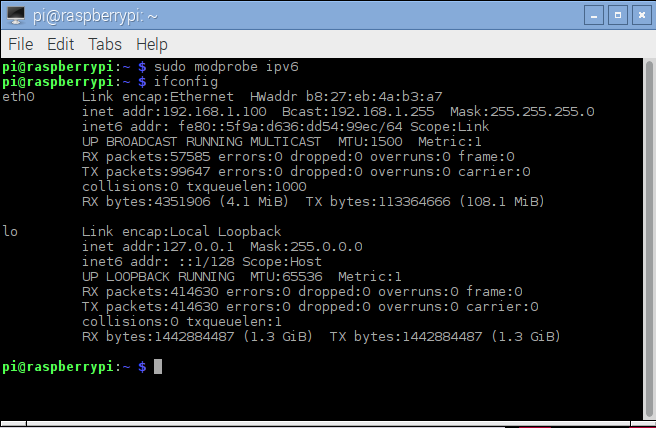
\includegraphics[scale=0.8]{ip6_1}   % Scale se utiliza para cambiar el tamaño de la imagen
			\caption{Configuración IPv6 raspberry pi}	
		\end{figure}
Para este caso en especifico la IPv6 es: \texttt{fe80::5f9a:d636:dd54:99ec} para comprobar podemos hacer un ping desde una pc que se encuentre en la red:

		\begin{figure}[H] 
			\centering
			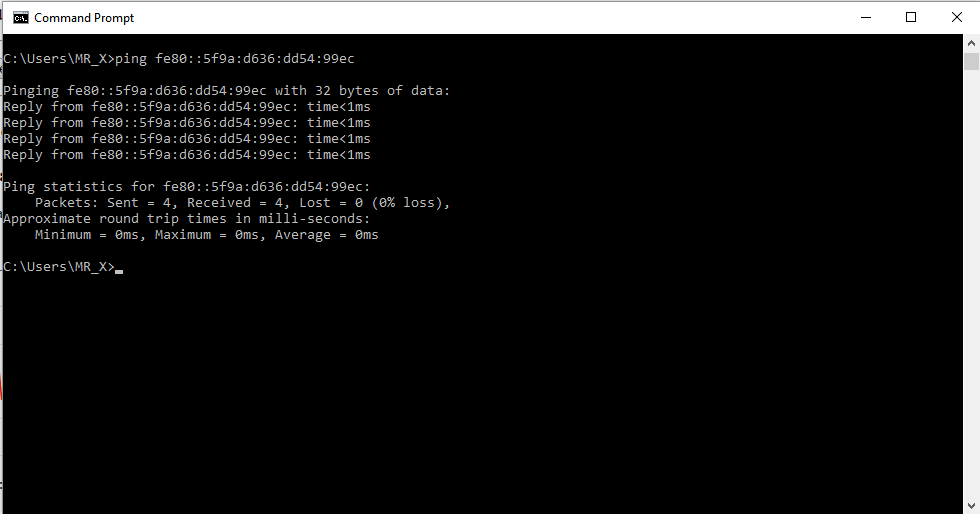
\includegraphics[scale=0.4]{ip6_2}  
			\caption{ping a la raspberry por protocolo IPv6 }	
		\end{figure}
Como ya se tiene la dirección IPv6 de la rasberry procedemos a configurarla en el servidor HTML que se va que se va a crear,, nos dirigimos a la carpeta \href{https://github.com/wilrilo/repo_final_nube/tree/master/repo_final_nube/ProyectoF_Pi/static/scripts}{\texttt{scripts}} que creamos previamente en la carpeta \texttt{static}, en ella abrimos un archivo llamado \href{https://github.com/wilrilo/repo_final_nube/blob/master/repo_final_nube/ProyectoF_Pi/static/scripts/raspberry.js}{raspberry.js} el cual llamará las variables del generadas en python a la pagina HTML, para ver el código completo de este archivo se puede ingresar al proyecto en hithub, en este archivo vamos a introducir la dirección IPv6 de la raspberry modificando la primera linea de código del archivo:

\begin{python}
	var ipDir = '//[fe80::5f9a:d636:dd54:99ec]:5000';  
\end{python} 
\subsubsection{pagina HTML}
En la carpeta \texttt{templates} creamos un archivo llamado \texttt{index.html} el cual tiene la pagina html que van a visualizar los usuarios de la red:

\begin{small}
	\begin{lstlisting}[frame=single]
<!doctype html>
<html lang="es">
<head>
<meta charset="UTF-8">
<title>Sistema para adquisicion de datos para el control y supervision de cultivos domesticos por protocolo IPV6</title>
<script src="//ajax.googleapis.com/ajax/libs/jquery/1.7.1/jquery.min.js" type="text/javascript"></script>
<script src="{{ static_url('scripts/raspberry.js') }}" type="application/javascript"></script>
</head>
<body>
<div>
<h1>Sistema para adquisicion de datos para el control y supervision de cultivos domesticos por protocolo IPV6</h1>
<p><span>Estado de la valvula: <span style="color: red;" id="estado">{{ estado }}</span></span></p>
</div>
<hr />
<input type="hidden" id="session" value="{{ session }}" />
<div id="led-on">
<p><input type="submit" value="Encender la valvula" id="add-button" /></p>
</div>
<div id="led-off" style="display: none;">
<p><input type="submit" value="Apagar la valvula" id="remove-button" /></p>
</div>
<hr />
<div>
<h2>Medicion de variables</h2>
<h3><span>Medidas de mi Sistema</span></h3>
<table border="2px">
<tr>
<td><p><span>Temperatura</span></p></td>
<td><p><span>Humedad</span></p>
</td>
</tr>
<tr>
<td><h2><iframe width="430" height="280" frameborder="0" src="https://app.ubidots.com/ubi/getchart/k_u4fOlasl9g0IsPvi6uHzqqgkg"></iframe></h2>
</td>
<td><h2><iframe width="430" height="280" frameborder="0" src="https://app.ubidots.com/ubi/getchart/uct647GdFRNHlosEX3_7LQ4Wx88"></iframe></h2>
</td>
</tr>
</table>
<h3><span>Medidas de los demas</span></h3>
<table border="2px">
<tr>
<td><p><span>Temperatura</span></p></td>
<td><p><span>Humedad</span></p>
</td>
</tr>
<tr>
<td><h2><<h2><iframe width="430" height="280" frameborder="0" src="https://app.ubidots.com/ubi/getchart/S862eWcAo1rArKC6IXQePIxw9fA"></iframe></h2>
</td>
<td><h2><iframe width="430" height="280" frameborder="0" src="https://app.ubidots.com/ubi/getchart/ltNyvhkOJGUaQtj_bMICPUKLI4E"></iframe></h2>
</td>
</tr>
</table>
</div>
</body>
</html>
	\end{lstlisting}
\end{small}	
Para obtener las frames de las variables de Ubidots nos vamos a la pagina de en \texttt{Dashboart} se vizualizan las variables que se han creado en la parte superior derecha de cualquiera de las variables, se hace clic  en la flecha para obtener los datos de la variable:

		\begin{figure}[H] 
			\centering
			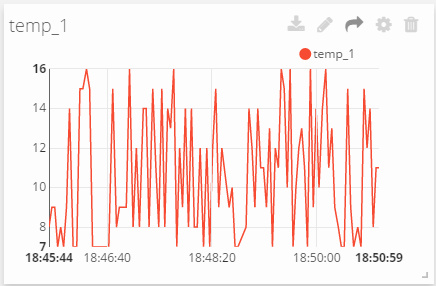
\includegraphics[scale=0.8]{html1}  
			\caption{compartir gráficos variables Ubidots para html}	
		\end{figure}

Finalmente copiamos el texto que aparece en el campo \textit{Add the following snippet to your HTML}, el cuadro que sale para compartir las gráficas también nos muestra la dirección UML de la gráfica de  \href{https://app.ubidots.com/ubi/getchart/page/k_u4fOlasl9g0IsPvi6uHzqqgkg}{temperatura}	
	
		\begin{figure}[H] 
			\centering
			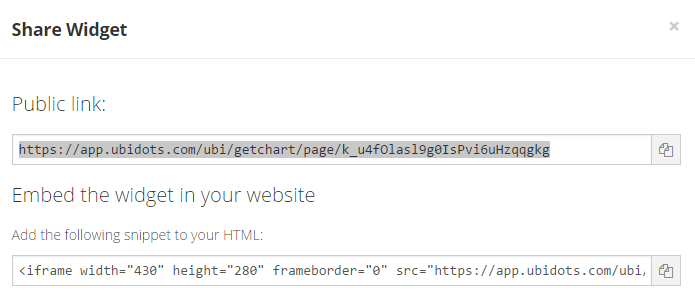
\includegraphics[scale=0.8]{html2}  
			\caption{compartir gráficos variables Ubidots para html}	
		\end{figure}

Finalmente la pagina para la visualización de los datos es la siguiente:

		\begin{figure}[H] 
			\centering
			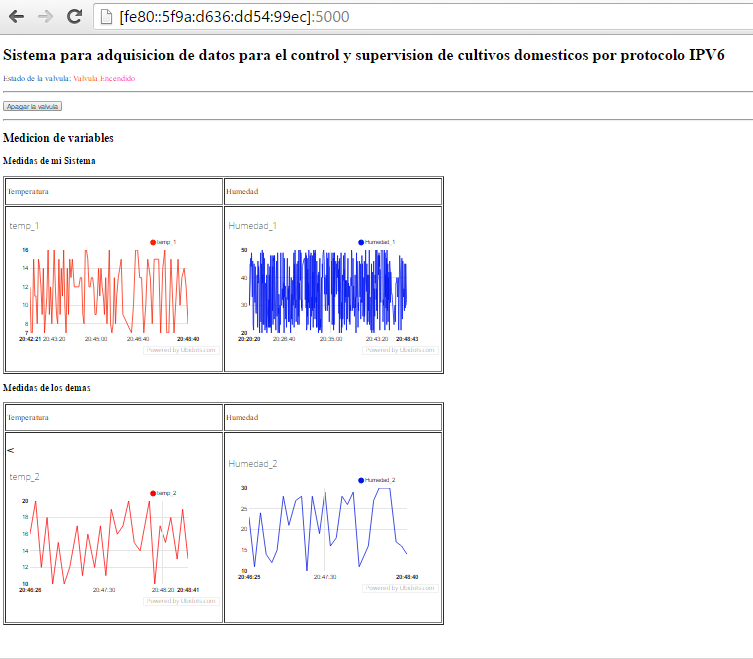
\includegraphics[scale=0.5]{html3}  
			\caption{pagina html}	
		\end{figure}

\subsection{Ejecución del programa}

Para la ejecución del proyecto abrimos una terminal en la raspberry, nos ubicamos en la carpeta donde desarrollamos el proyecto en este caso \href{https://github.com/wilrilo/repo_final_nube/tree/master/repo_final_nube/ProyectoF_Pi}{\texttt{proyectoF_Pi}} y escribimos el comando \texttt{python programa.py}:

		\begin{figure}[H] 
			\centering
			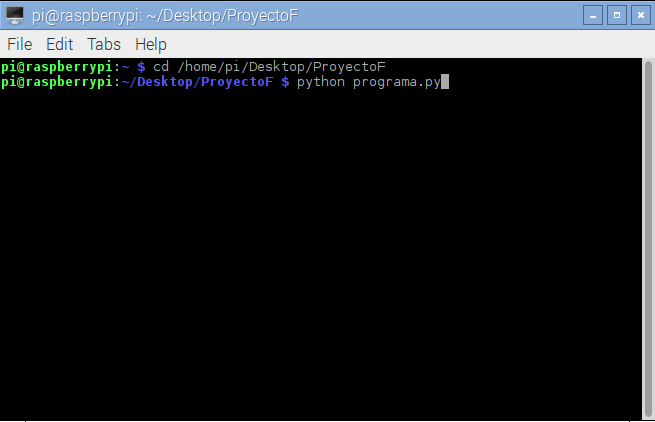
\includegraphics[scale=0.7]{eje1}  
			\caption{Comandos para ejecutar el programa}	
		\end{figure}

Al darle enter la consola comienza a mostrar las diferentes conexiones con la pagina de Ubidots para subir los datos: 

		\begin{figure}[H] 
			\centering
			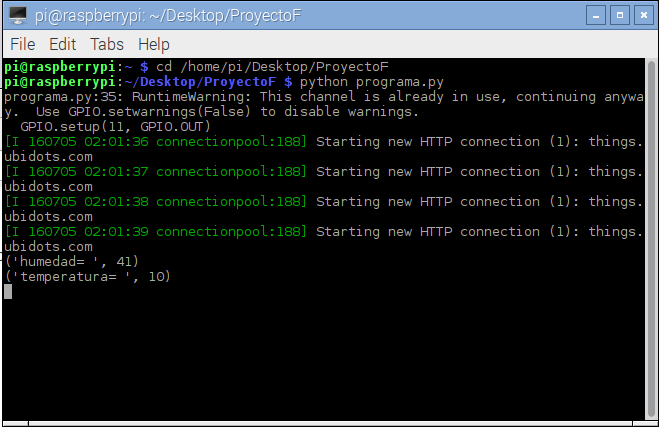
\includegraphics[scale=0.7]{eje2}  
			\caption{Programa ejecutándose en consola}	
		\end{figure}
		
Si entramos desde un dispositivo que se encuentre en la red a la dirección IPv6 de la raspberry al puerto 5000 observamos la pagina html que actualiza constantemente los datos que envía la raspberry: 

		\begin{figure}[H] 
			\centering
			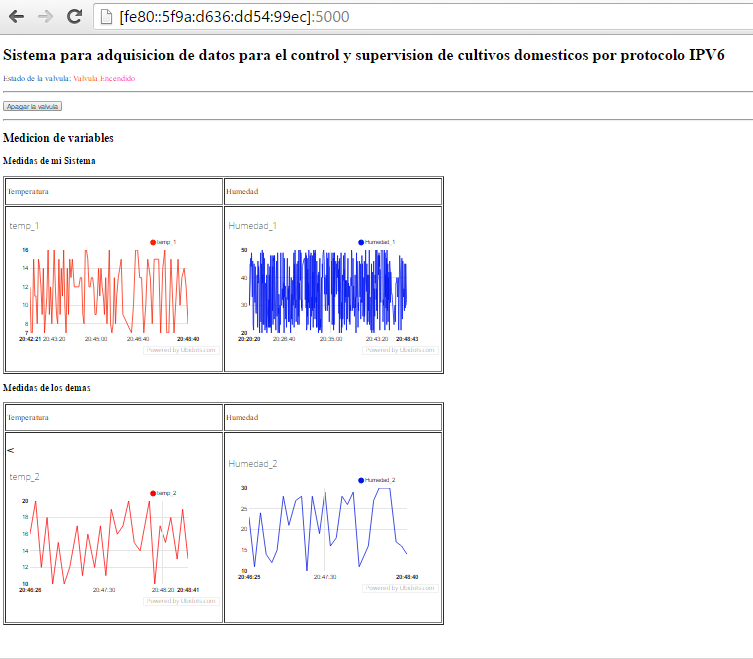
\includegraphics[scale=0.7]{html3}  
			\caption{pagina html}	
		\end{figure}

En la pagina se visualizan las 4 variables dos de temperatura y dos de humedad también se ve el estado de la válvula se puede encender y apagar desde la pagina o con un botón físico conectado a la raspberry.\\
Para verificar la conectividad entre dos dispositivos se creo un proyecto que se pudiese ejecutar en un computador con Ubuntu, el proyecto para PC se puede descargar de \href{https://github.com/wilrilo/repo_final_nube/tree/master/repo_final_nube/programaF_PC}{github}
 
 \subsection{Analisis de los datos }
 	
 En esta seccion se realizara un analisis estadistico de los datos por medio de R, como primer paso se instalan las siguientes librerías y paquetes 	
\begin{knitrout}
\definecolor{shadecolor}{rgb}{0.969, 0.969, 0.969}\color{fgcolor}\begin{kframe}
\begin{alltt}
\hlkwd{library}\hlstd{(methods)}
\hlkwd{library}\hlstd{(jsonlite)}
\end{alltt}
\end{kframe}
\end{knitrout}

Con estos dos paquetes Instalados podemos Descargar de la nube los datos generados por la Raspberry con los siguiente comandos:

\begin{knitrout}
\definecolor{shadecolor}{rgb}{0.969, 0.969, 0.969}\color{fgcolor}\begin{kframe}
\begin{alltt}
\hlstd{ubiURL}\hlkwb{<-}\hlstr{"http://things.ubidots.com/api/v1.6/variables/5763b2ab7625421ca1a7d82a/"}
\hlstd{ubiURL}\hlkwb{<-}\hlkwd{paste}\hlstd{(ubiURL,}\hlstr{"values/?token=SCJeJGv3tVyyiR9RjzBQXL9XgzCCxt"}\hlstd{,}\hlkwc{sep} \hlstd{=} \hlstr{""}\hlstd{)}
\end{alltt}
\end{kframe}
\end{knitrout}

En este caso hay que remplazar ID\_de\_la\_variable por el ID de cada variable y el \texttt{tokendeUbidots} por le token de la cuenta donde se encuentra la variable, la obtención de estos dos parámetros se explica en la sección llamada Ubidots. Ahora guardamos y separamos las diferentes variables que se descargan con \texttt{jsonlite}. 
\begin{knitrout}
\definecolor{shadecolor}{rgb}{0.969, 0.969, 0.969}\color{fgcolor}\begin{kframe}
\begin{alltt}
\hlstd{ubidots} \hlkwb{<-} \hlkwd{fromJSON}\hlstd{(ubiURL)}
\hlstd{valores} \hlkwb{<-} \hlstd{ubidots}\hlopt{$}\hlstd{results}\hlopt{$}\hlstd{value}
\hlstd{tiempos} \hlkwb{<-} \hlstd{ubidots}\hlopt{$}\hlstd{results}\hlopt{$}\hlstd{time}
\hlstd{marcas} \hlkwb{<-} \hlstd{ubidots}\hlopt{$}\hlstd{results}\hlopt{$}\hlstd{created}
\end{alltt}
\end{kframe}
\end{knitrout}

Ahora procedemos a realizar una gráfica de los datos obtenidos, para este graficamos la Humedad 1 :
 \begin{center}
\begin{knitrout}
\definecolor{shadecolor}{rgb}{0.969, 0.969, 0.969}\color{fgcolor}\begin{kframe}
\begin{alltt}
\hlkwd{plot}\hlstd{(tiempos,valores,}\hlstr{'l'}\hlstd{,}\hlkwc{col} \hlstd{=} \hlstr{"blue"}\hlstd{,}\hlkwc{main} \hlstd{=} \hlstr{"Datos de humedad 1"}\hlstd{)}
\end{alltt}
\end{kframe}
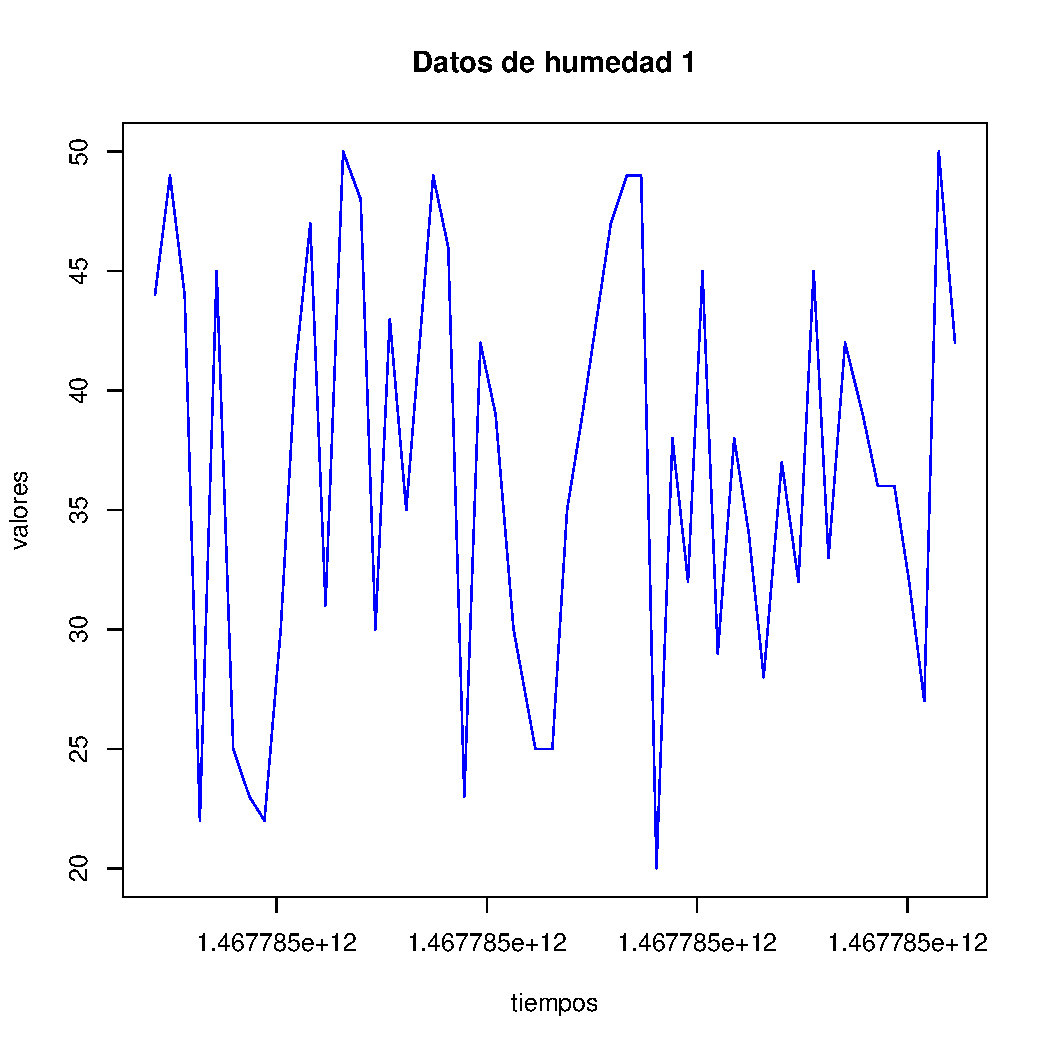
\includegraphics[width=4in]{figure/unnamed-chunk-4-1} 

\end{knitrout}
 \end{center}

 
También podemos realizar un estudio estadístico de los valores de la Humedad 1  
\begin{knitrout}
\definecolor{shadecolor}{rgb}{0.969, 0.969, 0.969}\color{fgcolor}\begin{kframe}
\begin{alltt}
\hlcom{#media}
\hlkwd{mean}\hlstd{(valores)}
\end{alltt}
\begin{verbatim}
## [1] 36.84
\end{verbatim}
\begin{alltt}
\hlcom{#mediana}
\hlkwd{median}\hlstd{(valores)}
\end{alltt}
\begin{verbatim}
## [1] 37.5
\end{verbatim}
\begin{alltt}
\hlcom{#cuartiles}
\hlkwd{quantile}\hlstd{(valores)}
\end{alltt}
\begin{verbatim}
##    0%   25%   50%   75%  100% 
## 20.00 30.00 37.50 44.75 50.00
\end{verbatim}
\begin{alltt}
\hlcom{#rango}
\hlkwd{range}\hlstd{(valores)}
\end{alltt}
\begin{verbatim}
## [1] 20 50
\end{verbatim}
\begin{alltt}
\hlcom{#varianza}
\hlkwd{var}\hlstd{(valores)}
\end{alltt}
\begin{verbatim}
## [1] 78.50449
\end{verbatim}
\begin{alltt}
\hlcom{#Desviacion estandar}
\hlkwd{sd}\hlstd{(valores)}
\end{alltt}
\begin{verbatim}
## [1] 8.860276
\end{verbatim}
\end{kframe}
\end{knitrout}

\begin{center}
\begin{knitrout}
\definecolor{shadecolor}{rgb}{0.969, 0.969, 0.969}\color{fgcolor}\begin{kframe}
\begin{alltt}
\hlkwd{boxplot}\hlstd{(valores,}\hlkwc{main}\hlstd{=}\hlstr{"Humedad_1"}\hlstd{,}\hlkwc{sub}\hlstd{=}\hlstr{"Grafico de caja"}\hlstd{,}\hlkwc{ylab}\hlstd{=}\hlstr{"humedad en %"}\hlstd{)}
\end{alltt}
\end{kframe}
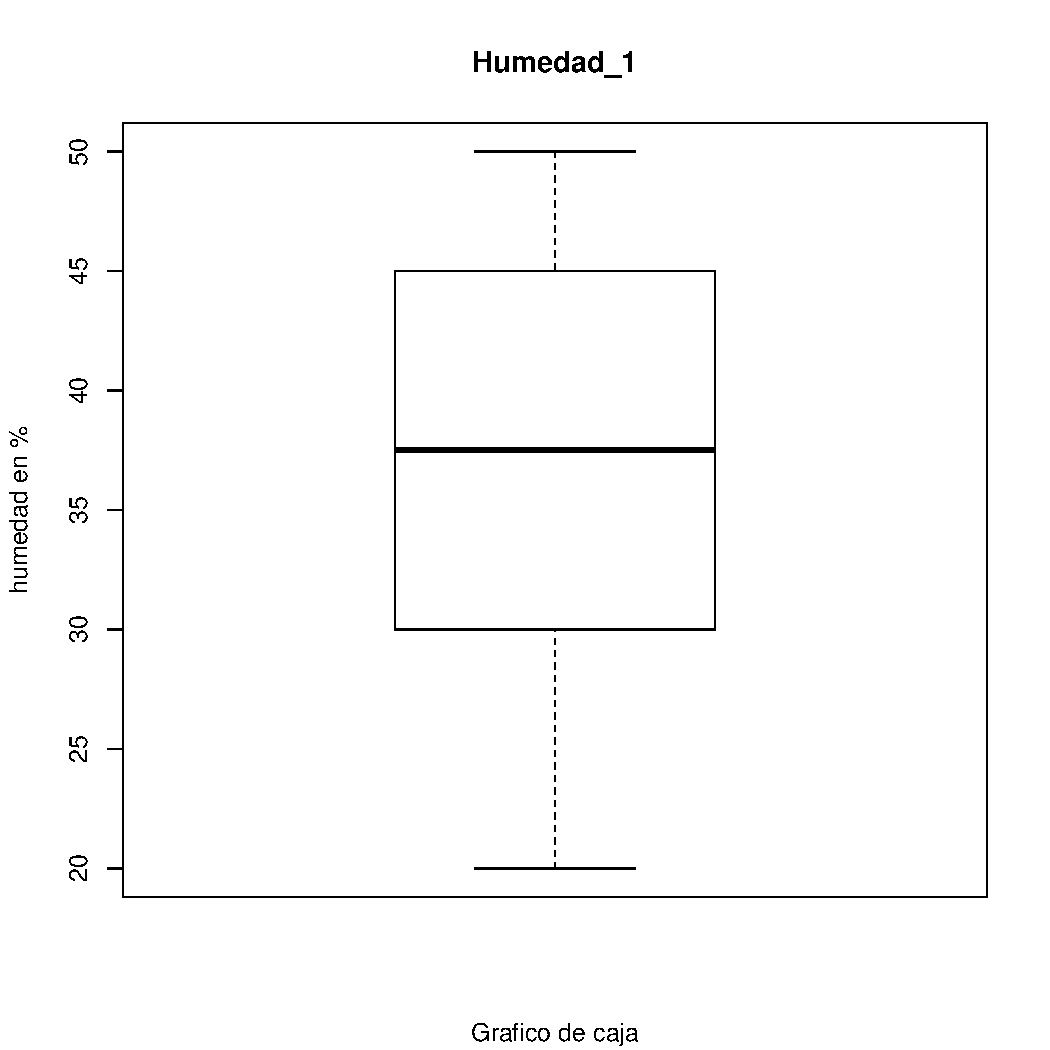
\includegraphics[width=3in]{figure/unnamed-chunk-6-1} 

\end{knitrout}
\end{center} 

Como parte Final de este trabajo se presentan las gráficas de las 4 variables que se manejaron se descargan y guardan todas las variables:
\begin{knitrout}
\definecolor{shadecolor}{rgb}{0.969, 0.969, 0.969}\color{fgcolor}\begin{kframe}
\begin{alltt}
\hlcom{#humedad 1}
\hlstd{ubiURL}\hlkwb{<-}\hlstr{"http://things.ubidots.com/api/v1.6/variables/5763b2c87625421f2f017764/"}
\hlstd{ubiURL}\hlkwb{<-}\hlkwd{paste}\hlstd{(ubiURL,}\hlstr{"values/?token=SCJeJGv3tVyyiR9RjzBQXL9XgzCCxt"}\hlstd{,}\hlkwc{sep} \hlstd{=} \hlstr{""}\hlstd{)}
\hlstd{ubidots1} \hlkwb{<-} \hlkwd{fromJSON}\hlstd{(ubiURL)}
\hlstd{hum1} \hlkwb{<-} \hlstd{ubidots}\hlopt{$}\hlstd{results}\hlopt{$}\hlstd{value}
\hlstd{thume1} \hlkwb{<-} \hlstd{ubidots}\hlopt{$}\hlstd{results}\hlopt{$}\hlstd{time}
\hlcom{#humedad 2}
\hlstd{ubiURL}\hlkwb{<-}\hlstr{"http://things.ubidots.com/api/v1.6/variables/5763b2c87625421f2f017764/"}
\hlstd{ubiURL}\hlkwb{<-}\hlkwd{paste}\hlstd{(ubiURL,}\hlstr{"values/?token=SCJeJGv3tVyyiR9RjzBQXL9XgzCCxt"}\hlstd{,}\hlkwc{sep} \hlstd{=} \hlstr{""}\hlstd{)}
\hlstd{ubidots2} \hlkwb{<-} \hlkwd{fromJSON}\hlstd{(ubiURL)}
\hlstd{hum2} \hlkwb{<-} \hlstd{ubidots}\hlopt{$}\hlstd{results}\hlopt{$}\hlstd{value}
\hlstd{thume2} \hlkwb{<-} \hlstd{ubidots}\hlopt{$}\hlstd{results}\hlopt{$}\hlstd{time}

\hlcom{#temperatura 1}
\hlstd{ubiURL}\hlkwb{<-}\hlstr{"http://things.ubidots.com/api/v1.6/variables/5763ac2376254249a1fa9eba/"}
\hlstd{ubiURL}\hlkwb{<-}\hlkwd{paste}\hlstd{(ubiURL,}\hlstr{"values/?token=SCJeJGv3tVyyiR9RjzBQXL9XgzCCxt"}\hlstd{,}\hlkwc{sep} \hlstd{=} \hlstr{""}\hlstd{)}
\hlstd{ubidots1} \hlkwb{<-} \hlkwd{fromJSON}\hlstd{(ubiURL)}
\hlstd{tem1} \hlkwb{<-} \hlstd{ubidots}\hlopt{$}\hlstd{results}\hlopt{$}\hlstd{value}
\hlstd{ttem1} \hlkwb{<-} \hlstd{ubidots}\hlopt{$}\hlstd{results}\hlopt{$}\hlstd{time}
\hlcom{#temperatura 2}
\hlstd{ubiURL}\hlkwb{<-}\hlstr{"http://things.ubidots.com/api/v1.6/variables/5763b35276254225fcaaa266/"}
\hlstd{ubiURL}\hlkwb{<-}\hlkwd{paste}\hlstd{(ubiURL,}\hlstr{"values/?token=SCJeJGv3tVyyiR9RjzBQXL9XgzCCxt"}\hlstd{,}\hlkwc{sep} \hlstd{=} \hlstr{""}\hlstd{)}
\hlstd{ubidots2} \hlkwb{<-} \hlkwd{fromJSON}\hlstd{(ubiURL)}
\hlstd{tem2} \hlkwb{<-} \hlstd{ubidots}\hlopt{$}\hlstd{results}\hlopt{$}\hlstd{value}
\hlstd{ttem2} \hlkwb{<-} \hlstd{ubidots}\hlopt{$}\hlstd{results}\hlopt{$}\hlstd{time}
\end{alltt}
\end{kframe}
\end{knitrout}

Ahora se muestran las cuatro variables en una gráfica:

\begin{center}
\begin{knitrout}
\definecolor{shadecolor}{rgb}{0.969, 0.969, 0.969}\color{fgcolor}\begin{kframe}
\begin{alltt}
\hlkwd{par}\hlstd{(}\hlkwc{mfrow}\hlstd{=}\hlkwd{c}\hlstd{(}\hlnum{2}\hlstd{,}\hlnum{2}\hlstd{))}
\hlkwd{plot}\hlstd{(thume1,hum1,}\hlstr{'l'}\hlstd{,}\hlkwc{col} \hlstd{=} \hlstr{"blue"}\hlstd{,}\hlkwc{main} \hlstd{=} \hlstr{"Datos de humedad 1"}\hlstd{)}
\hlkwd{plot}\hlstd{(thume2,hum2,}\hlstr{'l'}\hlstd{,}\hlkwc{col} \hlstd{=} \hlstr{"blue"}\hlstd{,}\hlkwc{main} \hlstd{=} \hlstr{"Datos de humedad 2"}\hlstd{)}
\hlkwd{plot}\hlstd{(ttem1,tem1,}\hlstr{'l'}\hlstd{,}\hlkwc{col} \hlstd{=} \hlstr{"red"}\hlstd{,}\hlkwc{main} \hlstd{=} \hlstr{"Datos de Temperatura 1"}\hlstd{)}
\hlkwd{plot}\hlstd{(ttem2,tem2,}\hlstr{'l'}\hlstd{,}\hlkwc{col} \hlstd{=} \hlstr{"red"}\hlstd{,}\hlkwc{main} \hlstd{=} \hlstr{"Datos de Temperatura 2"}\hlstd{)}
\end{alltt}
\end{kframe}
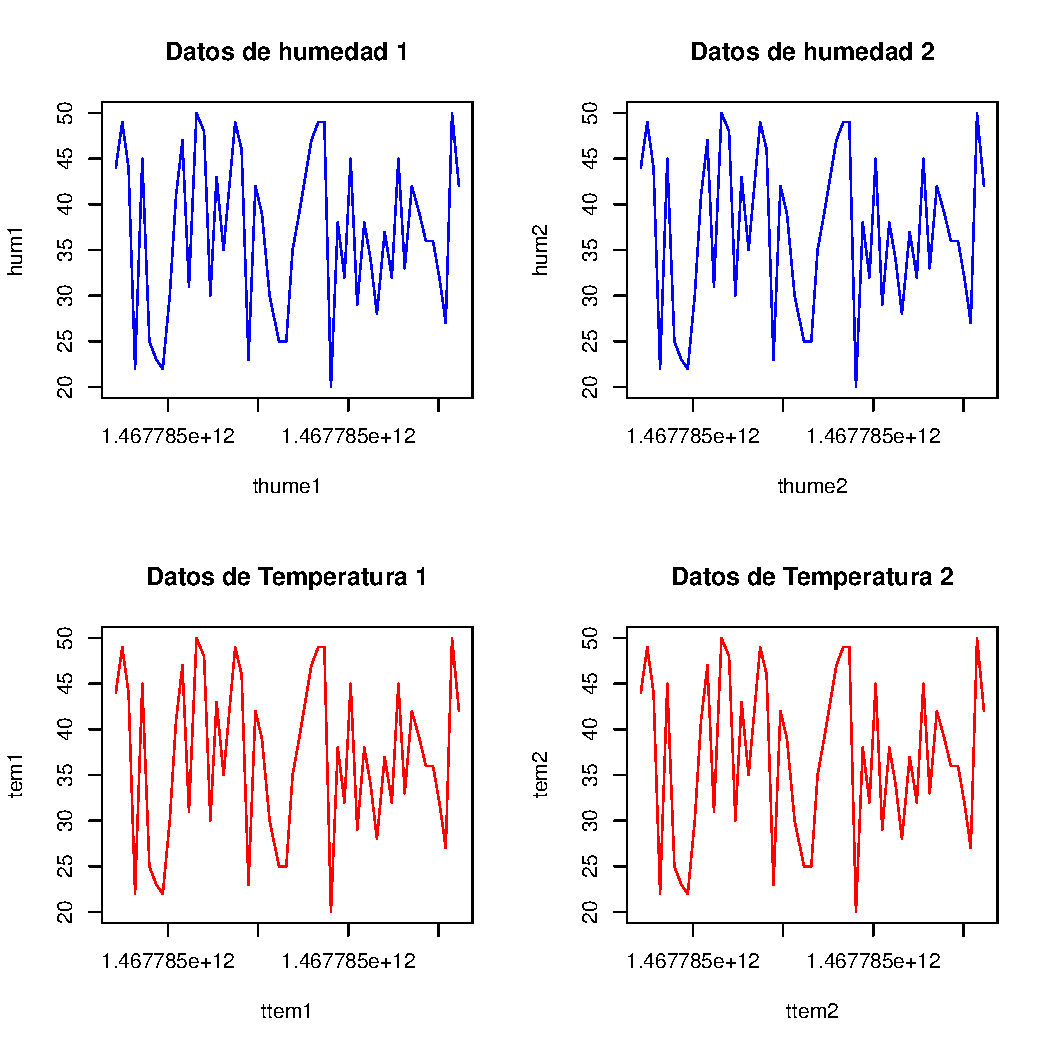
\includegraphics[width=3in]{figure/unnamed-chunk-8-1} 

\end{knitrout}
\end{center}	
 
 
 
 
\newpage		
		
	\textbf{{\Large Accesos WEB}}
	\begin{enumerate}
		\item  \href{http://silicio.mx/sensor-de-humedad-grove}{características sensor de humedad}
		\href{http://rita.udistrital.edu.co/index.php/servicios/servicios-internos/direccionamiento-ipv6-y-dns}{soporte rita IPv6}
		\item \href{	http://articulo.mercadolibre.com.mx/MLM-550669563-arduino-ethernet-shield-generico-atmel-robotica-_JMredirectedFromParent}{imagen arduino}
		\item \href{http://www.reflexiona.biz/shop/temperatura/559--sensor-de-temperatura-lm335a.html}{imagen sensor de temperatura}
		\item \href{http://www.atomsindustries.com/ASD1055}{imagen rasberry pi}
		
		\item \href{https://www.minagricultura.gov.co/}{ministerioagricultura}
		
		\item \href{http://ambientebogota.gov.co/techos-verdes-y-jardines-verticalessthash.tSdqSq1s.dpuf
			}{http://ambientebogota.gov.co/techos-verdes-y-jardines-verticalessthash.tSdqSq1s.dpuf [fecha de consulta: 22 de agosto de 2015]
			}
		
		\item \href{http://ambientebogota.gov.co/web/una-piel-natural-para-bogota//consulta-la-guia-tecnica-de-techos-}{http://ambientebogota.gov.co/web/una-piel-natural-para-bogota//consulta-la-guia-tecnica-de-techos-[fecha de consulta: 22 de agosto de 2015]}
		
		\item \href{http://www.eltiempo.com/colombia/cali/proyecto-vive-digital-llega-a-escuelas-de-narino/14681459}{http://www.eltiempo.com/colombia/cali/proyecto-vive-digital-llega-a-escuelas-de-narino/14681459[fecha de consulta: 22 de agosto de 2015]}
		
			\item \href{http://weblog.aklmedia.nl/tag/raspberry-pi/}{http://weblog.aklmedia.nl/tag/raspberry-pi/}
			

		%  
		
		%[13] 	%
		%
		%
		%[14]
		%verdes-para-bogota . 
		
		% granjasdigi
		%[15] http://www.eltiempo.com/colombia/cali/proyecto-vive-digital-llega-a-escuelas-de-narino/14681459 .
		%
		%[fecha de consulta: 22 de agosto de 2015]
		
		%% http://weblog.aklmedia.nl/tag/raspberry-pi/
	\end{enumerate}
	
	\bibliographystyle{apalike}						% Estilo de la bibliografía o referencias
	
	\bibliography{biblio}						% Se muestra desde el fichero .bbl
	
	
	
\end{document}
